\subsection{Concepto de función}

\begin{definition}
Una \emph{función entre dos conjuntos numéricos}, A conjunto inicial y B conjunto final, es una correspondencia por la cual a cada elemento de un subconjunto de A, llamado \emph{dominio de la función} y denotado por $Dom(f)$, le corresponde un elemento y sólo uno de un subconjunto de B, llamado \emph{imagen} o \emph{recorrido de f}, y denotado por $Im(f)$.\\
Una función se puede representar por:
$$f:A \rightarrow B$$
\end{definition}

Ejemplo de representación gráfica de una función:
\geogebra{bm9zpgfh}

\subsubsection{Clasificación de funciones}
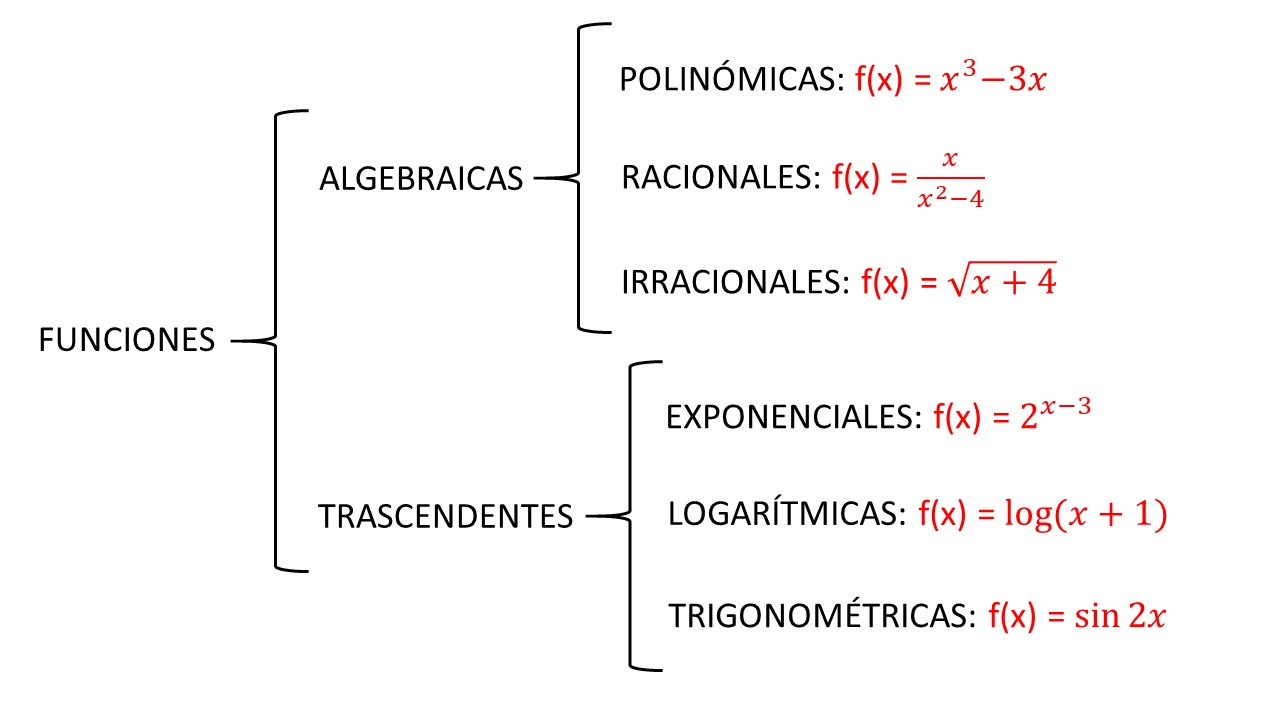
\includegraphics[width=40cm, height=20cm]{samples/propiedades/clasificaEsquema2.jpg}
\subsubsection{Ejemplos}
\begin{itemize}
	\item \textbf{Polinómicas.}
	$f(x) = x^3-3x$
	\geogebra{cwt7r5f7}
	\item \textbf{Racionales.}
	$f(x) = \dfrac{x}{x^2-4}$
	\geogebra{cdwjf88d}
	\item \textbf{Irracionales.}
	$f(x) = \sqrt{x+4}$
	\geogebra{xjn6vrn8}
	\item \textbf{Exponenciales.}
	$f(x) = 2^{x-3}$
	\geogebra{faj4urcm}
	\item \textbf{Logarítmicas.}
	$f(x) = \ln (x-1)$
	\geogebra{apzz89ae}
	\item \textbf{Trigonométricas.}
	$f(x) = \sin(2x)$
	\geogebra{yvw8jubg}
\end{itemize}

\subsubsection{Ejercicios.}
\begin{ex}[sol after]
	Rellene las siguientes definiciones:
		\begin{itemize}
			\item Una ............ es una relación entre dos conjuntos tal que a cada elemento del primer conjunto le corresponde ninguno, uno o varios elementos del segundo conjunto.
			\item Una \emph{función} es una ............. tal que a cada valor del ........ conjunto le corresponde un ......... valor del ........... conjunto.	
		\end{itemize}
	\begin{sol}
		\begin{itemize}
			\item Una \emph{correspondencia} es una relación entre dos conjuntos tal que a cada elemento del primer conjunto le corresponde ninguno, uno o varios elementos del segundo conjunto.
			\item Una función es una \emph{correspondencia} tal que a cada valor del \emph{primer} conjunto le corresponde un \emph{único} valor del \emph{segundo} conjunto. 
		\end{itemize}
	\end{sol}
\end{ex}


\begin{ex}[sol later]
	Introduzca en la barra de entrada las siguientes funciones, de manera similar a la indicada en el ejemplo anterior, y observa la gráfica de representación de cada una de las funciones.
	\begin{itemize}
		\item $f(x) = 3x+2$
		\item $g(x) = \dfrac{x^2-3}{x+5}$
		\item $h(x) = \sqrt{x+5}$
		\item $j(x) = \dfrac{2x^2+1}{3x-5}$
		\item $k(x) = \log (x^2)$
		\item $p(x) = 3\cos(3x)$
	\end{itemize}
	\begin{sol}
		\begin{itemize}
			\item $f(x) = 2x^3-3x$
			\item $f(x) = 6x+2$
			\item $f(x) = -\sqrt{x+1}$
			\item $f(x) = \tan (x-4)$
			\item $f(x) = \dfrac{2x-1}{x+7}$
			\item $f(x) = \log(x^2)$
		\end{itemize}
	\end{sol}
\end{ex}




\subsection{Dominio}

\begin{definition}
	El \emph{dominio de una función real}, también llamado \textbf{dominio de definición} o \textbf{campo de existencia}, es el conjunto de los elementos para los cuales la función está definida. Dicho de otra manera, es el subconjunto de números reales que tienen imagen.
	$$Dom_{f} =\{x \in R / \exists y = f(x) \in \mathbb{R}\}$$
\end{definition}
\begin{itemize} 
	\item $Dom_{f}$: dominio de la función. También se puede denotar por $Dom(f)$ o, simplemente, $D$. Puede ser todo el conjunto de los números reales, o buen un subconjunto de este: $Dom_{f} \subseteq R$. 
	\item $x$: número real, perteneciente al dominio de la función, que recibe el nombre de variable independiente. 
	\item $y$: número real, perteneciente al conjunto e la imagen de la función, recibe el nombre de variables dependiente. Para obtener su valor se debe aplicar la función $f$ al valor de $x: f(x)=y$. Para un par de valores concretos $(x,y)$ se dice que $y$ es la \textbf{imagen} de $x$, y que $x$ es la \textbf{antiimagen} de $y$.
\end{itemize} 
\youtube{lmfDEGDpgV8}
\subsubsection{Cómo calcular el dominio}
Para calcular el dominio "eliminaremos" de la ecuación aquellos valores que hagan imposible realizar alguna operación matemática.
\begin{itemize}
	\item \textbf{Funciones polinómicas}\\
	El dominio de toda función polinómica es R, ya que al sustituir un número real cualquiera $x \in R$, siempre va a existir $f(x)$.
	\item \textbf{Funciones racionales}\\
	El \textbf{denominador} debe de ser \textbf{diferente de cero}. Suponiendo una función $f(x) = \dfrac{P(x)}{Q(x)}$, si tanto $P(x)$ como $Q(x)$ son polinomios, entonces el dominio $Dom_{f}= \{x \in R / Q(x) \neq 0\}$, es decir, el conjunto de valores que \textbf{no anulan} el denominador.\\
	Cuando simplifiques una función racional, el dominio debe coincidir con el de la función original, y no debes caer en la tentación de recalcularlo.
	\item \textbf{Funciones irracionales}\\
	\begin{itemize}
		\item \emph{Función irracional de índice impar}\\
		En estos casos, la raíz no impone ninguna restricción adicional al dominio, por lo que coincidirá con el del radicando.
		\item \emph{Función irracional de índice par}\\
		En estos casos la raíz impone que los valores del radicando siempre sean mayores o iguales que cero.
	\end{itemize}
	\item \textbf{Funciones exponenciales}\\
	En estos casos, la exponencial no impone ninguna restricción adicional al dominio, con lo que coincidirá con el dominio del exponente.
	\item \textbf{Funciones logarítmicas}\\
	En estos casos el logaritmo impone que el argumento debe de ser un número positivo. 	
\end{itemize}
\subsubsection{Ejercicios}
\begin{ex}[sol later]
	Calcula el dominio de las siguientes funciones a partir de la teoría explicada previamente:\\
	\begin{itemize}
		\item $f(x) = \dfrac{2x}{3x-2}$
		\item $f(x) = \dfrac{6x}{x^2-16}$
		\item $f(x) = \sqrt{x^2-1}$
		\item $f(x) = \sqrt{\dfrac{3}{-x+2}}$
		\item $f(x) = \sqrt{\dfrac{x+5}{x-7}}$
		\item $f(x) = \sqrt{x^2+x}$
		\item $f(x) = \log(-2x^2-10x-8)$
		\item $f(x) = \arccos(x+5)$
		\item $f(x) = e^x$
		\item $f(x) = e^{-5x}$
	\end{itemize}
	\begin{sol}
		\begin{itemize}
			\item $\mathbb{R}-\{\dfrac{2}{3}\}$
			\item $\mathbb{R}-\{-4, 4\}$
			\item $(-\infty, -1]\bigcup [1, +\infty])$
			\item $(-\infty, 2)$
			\item $(-\infty, -5]\bigcup [7, +\infty])$
			\item $(-\infty, -1]\bigcup [0, +\infty])$
			\item $(-4,-1)$
			\item $[-6, -4]$
			\item $\mathbb{R}$
			\item $\mathbb{R}$
		\end{itemize}
	\end{sol}
\end{ex}

\vspace{1cm}

\begin{ex}[sol after]
	Comprueba mediante la representación en la gráfica que los dominios que has calculado coinciden con lo que se observa en las gráficas.
	\begin{sol}
		\geogebra[ai=true, stb=true]{tc5pbmae}
	\end{sol}
\end{ex}

\vspace{1cm}

\subsection{Simetría}

La gráfica de representación de una función puede presentar dos tipos de simetría: simetría respecto al eje de ordenadas o simetría respecto al origen de coordenadas. Veamos qué condiciones deben verificarse para que una función tenga alguno de estos tipos de simetría.
\youtube{UlD9kTKo7c8}
\subsubsection{Simetría respecto del eje de ordenadas}
\begin{definition}
	La gráfica de una función $f$ es \textbf{simétrica respecto del eje de ordenadas} si $f(x) = f(-x)$.
\end{definition}
Una función cuya gráfica es simétrica respecto del eje de ordenadas se denomina \textbf{función par}.\\
Por ejemplo, la función $f(x)=x^{2}$, es \textbf{simétrica respecto del eje de ordenadas}, puesto que:
$$f(x) = x^2 = (-x)^2 = f(-x)$$
\geogebra{cvscmh26}
\subsubsection{Simetría respecto del origen de coordenadas}
\begin{definition}
	La gráfica de una función $f$ es \textbf{simétrica respecto del origen de coordenadas} si $f(-x) = -f(x)$.
\end{definition}
Una función cuya gráfica es simétrica respecto del origen de coordenadas se denomina \textbf{función impar}.\\
Por ejemplo, la función $f(x)=x^{3}$, es \textbf{simétrica respecto del origen de coordenadas} ya que:
$$f(-x)=(-x)^3=-x^3=-f(x)$$
\geogebra{a4kksftu}
\youtube{kabnjBXPsWU}

\subsubsection{Ejercicios}
\begin{ex}[sol later]
	Estudia la simetría de las siguientes funciones indicando las operaciones que has realizado. Para ayudarte, puedes servirte de la representación gráfica de las mismas:\\
	\begin{itemize}
		\item $f(x) = 3x-x^3$
		\item $f(x) = x^4-2x^2-8$
		\item $f(x) = x^6+x^4-x^2$
		\item $f(x) = x^5+x^3-x$
		\item $f(x) = x \cdot |x|$
		\item $f(x) = |x| - 1$
		\item $f(x) = \dfrac{x^2}{1-x^2}$
		\item $f(x) = \dfrac{x}{1-x^2}$
		\item $f(x) = \dfrac{x^4+1}{x^2}$
		\item $f(x) = \dfrac{x^2}{2-x}$
	\end{itemize}
	\geogebra[ai=true, stb=true]{tc5pbmae}
	\begin{sol}
		\begin{itemize}
			\item $f(-x)=3(-x)-(-x^3)=-(3x-x^3)=-f(x) \rightarrow$ Función \textbf{simetría impar}
			\item $f(-x) = (-x)^4-2(-x)^2-8 = f(x) \rightarrow$ Función \textbf{simetría par}
			\item $f(-x) = (-x)^6+(-x)^4-(-x)^2 = x^6+x^4-x^2 = \rightarrow$ Función \textbf{simetría par}
			\item $f(-x) = (-x)^5+(-x^3)-(-x) = -x^5-x^3+x = -f(x) \rightarrow$ Función \textbf{simetría impar}
			\item $f(-x) = -x |x|= -x|x| = -f(x) \rightarrow$ Función \textbf{simetría impar}
			\item $f(-x) = |-x|-1 = |x|-1 = f(x) \rightarrow$ Función \textbf{simetría par}
			\item $f(-x)0\dfrac{(-x)^2}{1-(-x)^2} = \dfrac{x^2}{1-x^2} = f(x) \rightarrow$ Función \textbf{simetría par}
			\item $f(-x) = \dfrac{(-x)}{1-(-x)^2} = \dfrac{-x}{1-x^2} =-f(x) \rightarrow$ Función \textbf{simetría impar}
			\item $f(-x) = \dfrac{(-x)^4+1}{(-x)^2} = f(x) \rightarrow$ Función \textbf{simetría par}
			\item $f(-x) = \dfrac{(-x)^2}{2-(-x)} = \dfrac{x^2}{2+x} \rightarrow$ No presenta simetría
		\end{itemize}
	\end{sol}
\end{ex}

\vspace{1cm}


\begin{ex}[sol later]
	¿Qué tipo de simetría presentan las siguientes funciones?:\\
	\begin{itemize}
		\item $f(x) = x-1$
		\item $g(x) = \dfrac{1}{x}$
		\item $h(x) = \dfrac{x^2-4}{x^2+1}$
	\end{itemize}
	\geogebra{vyvhswrk}
	\begin{sol}
		\begin{itemize}
			\item $f(x) \rightarrow$ \textbf{no simétrica}
			\item $g(x) \rightarrow$ \textbf{simetría impar}
			\item $h(x) \rightarrow$ \textbf{simetría par}
		\end{itemize}
	\end{sol}
\end{ex}



\subsection{Periodicidad}

\begin{definition}
Una función es \textbf{periódica} de período $p$ si, para todo valor de $x$ perteneciente al dominio de la función, se verifica que $f(x+p)=f(x)$.
\end{definition}
\geogebra{bqzcquyw}
Si una función es periódica de período $p$, sus valores y, por tanto, su gráfica, se repiten en intervalos sucesivos de amplitud $p$.\\
Las funciones periódicas se estudian en un intervalo de amplitud $p$, y para construir el resto de la gráfica, solamente debemos de trasladar dicho estudio al resto del dominio de la función.
\youtube{dTgrxlz6bMs}
\subsubsection{Ejercicios}

\begin{scq}
	Selecciona la opción correcta:\\
	\begin{figure}
		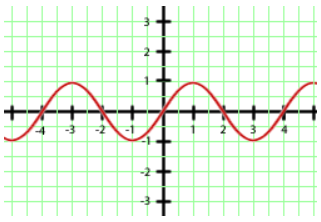
\includegraphics{samples/propiedades/periodicidad1.jpg}
	\end{figure}
	\begin{choices}
		\begin{choice}
			La función es periódica con periodo $T=2$.	
		\end{choice}
		\begin{choice}[x]
			La función es periódica con periodo $T=4$.
		\end{choice}	
		\begin{choice}
			La función no es periódica.
		\end{choice}
	\end{choices}
	\begin{feedback}
		Sus imágenes se repiten periódicamente en intervalos de longitud 4, por lo que la función es periódica con periodo $T=4$.
	\end{feedback}
\end{scq}

\vspace{1cm}


\begin{scq}
	Selecciona la opción correcta:\\
	\begin{figure}
		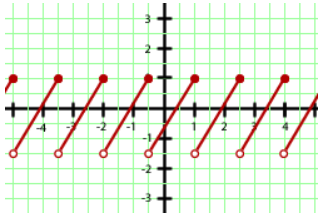
\includegraphics{samples/propiedades/periodicidad2.jpg}
	\end{figure}
	\begin{choices}
		\begin{choice}[x]s
			La función es periódica con periodo $T=2$.	
		\end{choice}
		\begin{choice}
			La función es periódica con periodo $T=4$.
		\end{choice}	
		\begin{choice}
			Ninguna de las respuestas anteriores es correcta.
		\end{choice}
	\end{choices}
	\begin{feedback}
		Sus imágenes se repiten periódicamente en intervalos de longitud 4, por lo que la función es periódica con periodo $T=2$.
	\end{feedback}
\end{scq}

\vspace{1cm}


\begin{scq}
	Selecciona la opción correcta:\\
	\begin{figure}
		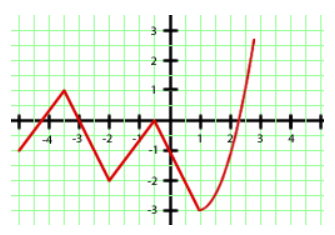
\includegraphics{samples/propiedades/periodicidad3.jpg}
	\end{figure}
	\begin{choices}
		\begin{choice}
			La función es periódica con periodo $T=5$.	
		\end{choice}
		\begin{choice}
			La función es periódica con periodo $T=6$.
		\end{choice}	
		\begin{choice}[x]
			La función no es periódica.
		\end{choice}
	\end{choices}
	\begin{feedback}
		No hay intervalos de igual longitud donde se repiten las imágenes, por lo que la función no es periódica.
	\end{feedback}
\end{scq}



\begin{scq}
	Selecciona la opción correcta:\\
	\begin{figure}
		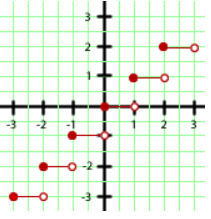
\includegraphics{samples/propiedades/periodicidad4.jpg}
	\end{figure}
	\begin{choices}
		\begin{choice}
			La función es periódica con periodo $T=1$.	
		\end{choice}
		\begin{choice}[x]
			La función es periódica con periodo $T=2$.
		\end{choice}	
		\begin{choice}[x]
			La función no es periódica.
		\end{choice}
	\end{choices}
	\begin{feedback}
		No hay intervalos de igual longitud donde se repiten las imágenes, por lo que la función no es periódica.
	\end{feedback}
\end{scq}



\begin{scq}
	Selecciona la opción correcta:\\
	\begin{figure}
		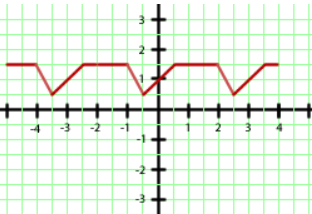
\includegraphics{samples/propiedades/periodicidad5.jpg}
	\end{figure}
	\begin{choices}
		\begin{choice}
			La función es periódica con periodo $T=-3$.	
		\end{choice}
		\begin{choice}[x]
			La función es periódica con periodo $T=3$.
		\end{choice}	
		\begin{choice}
			La función no es periódica.
		\end{choice}
	\end{choices}
	\begin{feedback}
		Sus imágenes se repiten periódicamente en intervalos de longitud 3, por lo que la función es periódica con periodo $T=3$.
	\end{feedback}
\end{scq}


\subsection{Puntos de corte con los ejes}

Si una función corta el \textbf{eje de abscisas}, lo hace en los puntos $(x, 0)$, es decir, los puntos donde $f(x)=0$.\\
\\
Si una función corta el \textbf{eje de ordenadas}, lo hace en el punto $(0, f(0))$, si $0$ pertenece al dominio de la función.\\
\\
Una función puede cortar el eje de abscisas varias veces, una vez o ninguna, pero no puede cortar el eje de ordenadas en más de un punto, dado que en dicho caso no sería una función.\\
\\
Para calcular los puntos de corte con el eje de abscisas, se debe de igualar la función a $0$. Siendo el valor obtenido el valor de la $x$ y el 0 el valor de la $y$. En el caso de los puntos de corte del eje de ordenadas, para calcular el valor de la $y$ correspondiente al punto que posee $x=0$, se debe de calcular el valor de la función en $0$, $y=f(0)$.\\
\youtube{FnauclNt3do}
\subsubsection{Signo de una función}
Determinar el signo de una función consiste en hallar las zonas donde la función está por encima o por debajo del eje de abscisas, es decir, los valores del dominio para los cuales $f(x) > 0$ o $f(x) < 0$ .\\
\\
Para determinar el signo de la función debemos representar en el eje de abscisas los puntos de corte de la función con dicho eje y los puntos donde la función no está definida. Después, analizamos el signo de la función en los distintos trozos.
\subsubsection{Ejercicios}

\begin{ex}[sol later]
	Determina los puntos de corte con los ejes de la función $f(x)=x^2$
	\begin{sol}
		El punto de corte con los ejes es: $(0,0)$
		\geogebra{un6xmbsf}
	\end{sol}
\end{ex}

\vspace{1cm}

\begin{ex}[sol later]
	Determina los puntos de corte con los ejes de la función $f(x)=\dfrac{3x^2}{x^2+1}$
	\begin{sol}
		El punto de corte con los ejes es: $(0,0)$
		\geogebra{fd2tfayt}
	\end{sol}
\end{ex}

\vspace{1cm}

\begin{ex}[sol later]
	Determina los puntos de corte con los ejes de la función $f(x)=x^4-2x^2$
	\begin{sol}
		Los puntos de corte con los ejes son $(0,0), (\sqrt{2}, 0)$ y $(-\sqrt{2}, 0)$
		\geogebra{e4fb746d}
	\end{sol}
\end{ex}

\vspace{1cm}

\begin{ex}[sol later]
	Determina los puntos de corte con los ejes de la función $f(x)=\sqrt{x^2-1}$
	\begin{sol}
		Los puntos de corte con los ejes son $(1, 0)$ y $(-1, 0)$
		\geogebra{mrr3hqe8}
	\end{sol}
\end{ex}

\vspace{1cm}

\begin{ex}[sol later]
	Determina los puntos de corte con los ejes de la función $f(x)=\dfrac{1}{x^2-9}$
	\begin{sol}
		El punto de corte con los ejes es: $(0,-\dfrac{1}{9})$
		\geogebra{cfme2yq3}
	\end{sol}
\end{ex}

\vspace{1cm}





\begin{ex}[sol later]
	Determina los puntos de corte con los ejes de la función que se muestra a continuación:\\
	\geogebra{mvmuqk5u}
	\begin{sol}
		El punto de corte con los ejes es: $(0,1)$
	\end{sol}
\end{ex}

\vspace{1cm}

\begin{ex}[sol later]
	Determina los puntos de corte con los ejes de la función que se muestra a continuación:\\
	\geogebra{d4audnb2}
	\begin{sol}
		No hay puntos de corte con los ejes.
	\end{sol}
\end{ex}

\vspace{1cm}

\begin{ex}[sol later]
	Determina los puntos de corte con los ejes de la función que se muestra a continuación:\\
	\geogebra{mv8baxdm}
	\begin{sol}
		No hay puntos de corte con los ejes.
	\end{sol}
\end{ex}

\vspace{1cm}

\begin{ex}[sol later]
	Determina los puntos de corte con los ejes de la función que se muestra a continuación:\\
	\geogebra{kcbmtz7k}
	\begin{sol}
		El punto de corte con los ejes es: $(0,0)$
	\end{sol}
\end{ex}

\vspace{1cm}

\begin{ex}[sol later]
	Determina los puntos de corte con los ejes de la función que se muestra a continuación:\\
	\geogebra{fw3xywww}
	\begin{sol}
		El punto de corte con los ejes es: $(0,0)$
	\end{sol}
\end{ex}


\subsection{Crecimiento y decrecimiento}
\begin{definition}
	Una función $f$ es \textbf{creciente} en un intervalo si para cualesquiera $x_1$ y $x_2$ del intervalo tales que $x_{1} < x_{2}$, se verifica que $f(x_{1}) \leq f(x_{2})$.
\end{definition}
Si la desigualdad es estricta, es decir, si para cualesquiera $x_1$ y $x_2$ tales que $x_1 < x_2$ se verifica que $f(x_{1}) < f(x_{2})$, la función es \textbf{estrictamente creciente}.\\
\newline
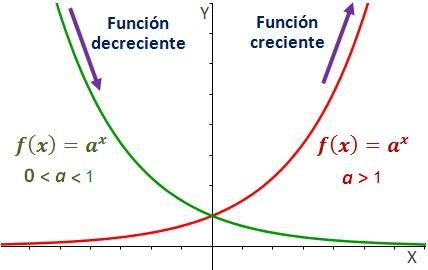
\includegraphics{samples/propiedades/crecienteDecreciente.jpg}\\
\begin{definition}
	Una función $f$ es \textbf{decreciente} en un intervalo si para cualesquiera $x_1$ y $x_2$ del intervalo tales que $x_{1} < x_{2}$, se verifica que $f(x_{1}) \geq f(x_{2})$.	
\end{definition}
Como en el caso anterior, si para cualesquiera $x_1$ y $x_2$ tales que $x_{1} < x_{2}$ se verifica que $f(x_{1}) > f(x_{2})$, la función es \textbf{estrictamente decreciente}.\\
\youtube{cWqJfem3GTk}
\subsubsection{Ejercicios}

\begin{ex}[sol later]
	Determina los intervalos de crecimiento y decrecimiento de la función $f(x)=x^4-2x^2-8$
	\begin{sol}
		\begin{itemize}
			\item Crecimiento: $(-1,0) \bigcup (1,+\infty)$
			\item Decrecimiento: $(-\infty, -1) \bigcup (0,1)$
		\end{itemize}
		\geogebra{rahsjufx}
	\end{sol}
\end{ex}

\vspace{1cm}

\begin{ex}[sol later]
	Determina los intervalos de crecimiento y decrecimiento de la función $f(x)=3x^4-20x^3-6x^2+60x-8$
	\begin{sol}
		\begin{itemize}
			\item Crecimiento: $(-1,1) \bigcup (5, +\infty)$
			\item Decrecimiento: $(-\infty, -1) \bigcup (1,5)$
		\end{itemize}
		\geogebra{z2jageyv}
	\end{sol}
\end{ex}

\vspace{1cm}

\begin{ex}[sol later]
	Determina los intervalos de crecimiento y decrecimiento de la función $f(x)=\dfrac{x+1}{x^2+x-2}$
	\begin{sol}
		\begin{itemize}
			\item Decrecimiento: $\mathbb{R}-\{-2,1\}$ 
		\end{itemize}
		\geogebra{zjmqndnw}
	\end{sol}
\end{ex}

\vspace{1cm}

\begin{ex}[sol later]
	Determina los intervalos de crecimiento y decrecimiento de la función $f(x)=\dfrac{x^4+1}{x^2}$
	\begin{sol}
		\begin{itemize}
			\item Crecimiento: $(-1,0) \bigcup (1, +\infty)$
			\item Decrecimiento: $(-\infty, -1) \bigcup (0,1)$ 
		\end{itemize}
		\geogebra{ct2hh9nx}
	\end{sol}
\end{ex}

\vspace{1cm}

\begin{ex}[sol later]
	Determina los intervalos de crecimiento y decrecimiento de la función $f(x)=\dfrac{x}{1+x^2}$
	\begin{sol}
		\begin{itemize}
			\item Crecimiento: $(-1,1)$
			\item Decrecimiento: $(-\infty, -1) \bigcup (1, +\infty)$ 
		\end{itemize}
		\geogebra{m6jd6rcj}
	\end{sol}
\end{ex}

\vspace{1cm}

\begin{ex}[sol later]
	Trata de observar los intervalos de crecimiento y de crecimiento de las siguientes funciones ayudándote de la representación gráfica de las mismas:
	\begin{itemize}
		\item $f(x) = x + \sqrt{x}$
		\item $f(x) = e^{\dfrac{1}{x}}$
		\item $f(x) = (x-1)e^{-x}$
		\item $f(x) = \dfrac{\ln(x)}{x}$
	\end{itemize}
	\geogebra[stb=true, ai=true]{tc5pbmae}
	\begin{sol}
		Juega con el applet de Geogebra.
	\end{sol}
\end{ex}


\subsection{Máximos y mínimos relativos y absolutos}
\begin{definition}
	Una función tiene un \textbf{máximo relativo} en $x=a$ si para todo $x$ de un entorno de $a$ se verifica que $f(a)$ es mayor o igual que $f(x)$.
\end{definition}

\begin{definition}
	Una función tiene un \textbf{mínimo relativo} en $x=a$ si para todo $x$ de un entorno de $a$ se verifica que $f(a)$ es menor o igual que $f(x)$.
\end{definition}

\begin{definition}
	Una función tiene un \textbf{máximo(mínimo) absoluto} en $x=a$ si para todo $x$ ded $Dom (f)$ se verifica que $f(a)$ es mayor(menor) o igual que $f(x)$.
\end{definition}

En la siguiente función, se puede observar cuales son los máximos y los mínimos relativos.
\geogebra{bxmrfp5r}
\subsubsection{Ejercicios}
\begin{ex}[sol later]
	Clacula los máximos y los mínimos de las siguientes funciones:\\
	\begin{itemize}
		\item \geogebra{uxmbmw2k}
		\item \geogebra{mubhyvzv}
		\item \geogebra{whfwaz4t}
	\end{itemize}
	\begin{sol}
		\begin{itemize}
			\item Máximo: $(0,0)$
			\item No presenta ni máximos ni mínimos.
			\item Máximo: $(1,3)$ \\ Mínimo: $(3,-1)$
		\end{itemize}
	\end{sol}
\end{ex}

\vspace{1cm}

\begin{ex}[sol later]
	Calcula los máximos y los mínimos de las siguientes funciones:\\
	\begin{itemize}
		\item $f(x)=x^3-3x^2+3$
		\geogebra{kesnfpdm}
		\item $f(x)=3x^4-4x^3$
		\geogebra{v7cynn2w}
		\item $f(x)=\dfrac{3}{x^2+1}$
		\geogebra{g6kcsfkb}
	\end{itemize}
	\begin{sol}
		\begin{itemize}
			\item Máximo en $x=0$ y mínimo en $x=2$.
			\item Mínimo en $x=1$.
			\item Máximo en $x=0$.
		\end{itemize}
	\end{sol}
\end{ex}


\subsection{Concavidad y puntos de inflexión}
\begin{definition}
Un \textbf{punto de inflexión} de una función es un punto en el que la función cambia de convexa $(\bigcup)$ a cóncava $(\bigcap)$, o viceversa, y la tangente atraviesa la gráfica.
\end{definition}
A continuación se muestra un ejemplo de punto de inflexión.
\geogebra{kzzn4gj2}


\begin{definition}
Estudiar la \textbf{curvatura} de una función consiste en estudiar en qué intervalos es convexa $(\bigcup)$ y en cuáles es cóncava $(\bigcap)$. Los intervalos de curvatura están separados por los puntos de inflexión y las discontinuidades.
\end{definition}

\subsubsection{Ejercicios}
\begin{ex}[sol later]
	Calcula los puntos de inflexión de las siguientes funciones:\\
	\begin{itemize}
		\item $f(x)=-x^3+3x$
		\geogebra{tkhxm6jf}
	\end{itemize}
	\begin{sol}
		\begin{itemize}
			\item Punto de inflexión en $(0,0)$.
		\end{itemize}
	\end{sol}
\end{ex}





\subsection{Operaciones con funciones}

Sean dos funciones $f$ y $g$ definidas en el mismo subconjunto $D$ de los números reales, se definen las siguientes operaciones entre ellas:
\begin{itemize}
	\item \textbf{Adición}: la suma de $f$ y $g$ es la función $f+g$ que, para cualquier $x \in D$, verifica:
	$$(f+g)(x) = f(x)+g(x)$$
	\item \textbf{Sustracción}: la diferencia de $f$ y $g$ es la función $f-g$ que, para cualquier $x \in D$, verifica:
	$$(f-g)(x) = f(x)-g(x)$$
	\item \textbf{Multiplicación}: el producto de $f$ y $g$ es la función $f \cdot g$ que, para cualquier $x \in D$, verifica:
	$$(f \cdot g)(x) = f(x) \cdot g(x)$$
	\item \textbf{División}: el cociente de $f$ y $g$ es la función $\frac{f}{g}$ que, para cualquier $x \in D$, con $g(x) \neq 0$, verifica:
	$$(\dfrac{f}{g})(x) = \dfrac{f(x)}{g(x)}$$
\end{itemize}
Las operaciones con funciones verifican las mismas propiedades que las operaciones con números reales, ya que se definen utilizando las operaciones con sus imágenes, que son números reales.\\
El dominio de las funciones $f+g$, $f-g$, $f \cdot g$ y $\dfrac{f}{g}$ es la intersección de los dominios de $f$ y $g$, con la salvedad de que en el caso $\dfrac{f}{g}$, los valores de x que anulan el denominador no pertenecen al dominio.\\

\begin{itemize}
	\item \textbf{EJEMPLO}
                  \\
	\youtube{jP1mSfUqpxw}
\end{itemize}


\subsubsection{Ejercicios}

\begin{ex}[sol later]
	Dadas las funciones $f(x)=5x+6$ y $g(x)=3x^2-4x+8$, calcula la suma $(f+g)(x)$ y la resta $(f-g)(x)$ de las funciones.
	\begin{sol}
		\begin{itemize}
			\item $(f+g)(x) = f(x)+g(x) = (5x+6)+(3x^2-4x+8) = 3x^2+x+14$
			\item $(f-g)(x) = f(x)-g(x) = (5x+6)-(3x^2-4x+8) = -3x^2+9x-2$
		\end{itemize}
	\end{sol}
\end{ex}

\vspace{1cm}

\begin{ex}[sol later]
	Dadas las funciones $f(x)=12x^3+15x^2-6x$ y $g(x)=3x$, calcula el producto $(f \cdot g)(x)$ y la división $(\dfrac{f}{g})(x)$ de las funciones.
	\begin{sol}
		\begin{itemize}
			\item $(f \cdot g)(x) = f(x) \cdot g(x) = (12x^3+15x^2-6x) \cdot(3x) = 36x^4+45x^3-18x^2$
			\item $(\dfrac{f}{g})(x) = \dfrac{f(x)}{g(x)} = \dfrac{(12x^3+15x^2-6x)}{(3x)} = 4x^2+5x-2$
		\end{itemize}
	\end{sol}
\end{ex}

\vspace{1cm}

\begin{ex}[sol later]
	Dadas las funciones $f(x)=\sqrt{x}$, $g(x)=x-4$ y $h(x)=\dfrac{2}{3-x}$, calcula
	\begin{itemize}
		\item $(f+g)(x)$
		\item $(g+h)(x)$
		\item $(\dfrac{f}{g})(x)$
		\item $(\dfrac{g}{f})(x)$
		\item $(f\cdot g)(x)$
		\item $(\dfrac{g}{h})(x)$
	\end{itemize} 
	\begin{sol}
		\begin{itemize}
			\item $(f+g)(x) = f(x) + g(x) = \sqrt{x} + (x-4) = \sqrt{x} + x -4$
			\item $(g+h)(x) = g(x) + h(x) = (x-4) + \dfrac{2}{3-x} = x - 4 + \dfrac{2}{3-x}$
			\item $(\dfrac{f}{g})(x) = \dfrac{f(x)}{g(x)} = \dfrac{\sqrt{x}}{x-4}$
			\item $(\dfrac{g}{f})(x) = \dfrac{g(x)}{f(x)} = \dfrac{x-4}{\sqrt{x}}$
			\item $(f\cdot g)(x) = f(x) \cdot g(x) = \sqrt{x} \cdot \dfrac{2}{3-x} = \dfrac{2\sqrt{x}}{3-x}$
			\item $(\dfrac{g}{h})(x) = \dfrac{g(x)}{h(x)} = \dfrac{x-4}{\dfrac{2}{3-x}} = \dfrac{(x-4)(3-x)}{2}$
		\end{itemize}
	\end{sol}
\end{ex}


\subsection{Función compuesta}

\begin{definition}
Dadas dos funciones $f$ y $g$, la \emph{función compuesta} de $f$ y $g$, que se simboliza con $g \circ f$, es la función que transforma $x$ en $g(f(x))$.
$$ x \rightarrow f(x) \rightarrow g(f(x))$$
El dominio de la función compuesta $g \circ f$ está formada por los valores de $x$ pertenecientes al dominio de $f$ tales que $f(x)$ pertenece al dominio de $g$.
$$Dom(f \circ g) = Dom(f)$$
\end{definition}
Por ejemplo, si $f(x) = 3x - 1$ y $g(x) = \dfrac{1}{x^{2}+1}$, entonces la función compuesta $f$ y $g$ es $$(g \circ f)(x) = g(f(x)) = g(3x-1) = \dfrac{1}{(3x-1)^{2}+1}$$.\\
También podemos considerar la función compuesta de $g$ y $f$:
$$(f \circ g)(x) = f(g(x)) = f(\dfrac{1}{x^2 + 1}) = 3 \cdot \dfrac{1}{x^2 + 1} - 1$$
En general, la composición de funciones no es una operación conmutativa. Es decir, $g \circ f \neq f \circ g$, excepto en algunos casos particulares. Además, se puede dar el caso de que alguna de las dos funciones compuestas no exista.
\youtube{v8j1qoTvDSg}
\subsubsection{Propiedades}
Las propiedades más características de la composición de funciones son la propiedad asociativa y la propiedad no conmutativa.
\begin{itemize}
	\item \textbf{Propiedad asociativa.} Tres funciones cualesquiera $f$, $g$, $h$, que se pueden componer, verifican:
	$$h \circ (g \circ f) = (h \circ g) \circ f$$
	\item \textbf{Propiedad no conmutativa.} La composición de funciones, en general, no es conmutativa.
	$$g \circ f \neq f \circ g$$
\end{itemize}

\begin{ex}[sol later]
	Sean $f(x)=3x+2$ y $g(x)=\dfrac{x+3}{2x+1}$, calcula $(g \circ f)$ y $(f \circ g)$.
	\begin{sol}
		\begin{itemize}
			\item $g \circ f = g[f(x)] = g(3x+2) = \dfrac{3x+2+3}{2(3x+2)+1} = \dfrac{3x+5}{6x+5}$
			\item $f \circ g = f[g(x)] = f(\dfrac{x+3}{2x+1}) = 3\dfrac{x+3}{2x+1} + 2=\dfrac{7x+11}{2x+1}$
		\end{itemize}
	\end{sol}
\end{ex}

\vspace{1cm}


\begin{ex}[sol later]
	Sean $f(x)=\dfrac{x+2}{2x+1}$ y $g(x)=\sqrt{x}$, calcula $g \circ f$ y $f \circ g$.
	\begin{sol}
		\begin{itemize}
			\item $g \circ f = g[f(x)] = g(\dfrac{x+2}{2x+1}) = \sqrt{\dfrac{x+2}{2x+1}}$
			\item $f \circ g = f[g(x)] = f(\sqrt{x}) =\dfrac{\sqrt{x}+2}{2\sqrt{x}+1}$
		\end{itemize}
	\end{sol}
\end{ex}

\vspace{1cm}

\begin{ex}[sol later]
	Sean $f(x)=\dfrac{1}{2x-1}$, $g(x)=\dfrac{2x-1}{2x+1} \text{ y } h(x)=\dfrac{1}{x}$, calcula $g \circ f$, $f \circ g$, $h \circ g \circ f$ y $h \circ f \circ g$.
	\begin{sol}
		\begin{itemize}
			\item $g \circ f = g[f(x)] = g(\dfrac{1}{2x-1}) = \dfrac{2(\dfrac{1}{2x-1})-1}{2(\dfrac{1}{2x-1})+1} = \dfrac{3-2x}{2x+1}$
			\item $f \circ g = f[g(x)] = f(\dfrac{2x-1}{2x+1}) =\dfrac{1}{2(\dfrac{2x-1}{2x+1})-1} = \dfrac{2x+1}{2x-3}$
			\item $h \circ g \circ f= h[(g \circ f)(x)] = h(\dfrac{3-2x}{2x+1}) = \dfrac{2x+1}{3-2x}$
			\item $h \circ f \circ g= h[(f \circ g)(x)] = h(\dfrac{2x+1}{2x-3}) = \dfrac{2x-3}{2x+1}$
		\end{itemize}
	\end{sol}
\end{ex}



\subsection{Función inversa}

\begin{definition}
Dada una función $f$, se denomina \emph{función inversa} de $f$, si existe, y se simboliza con $f^{-1}$, la función que cumple:
$$f^{-1}(y) = x \longleftrightarrow f(x) = y$$
\end{definition}
La función inversa de $f^{-1}$ es, a su vez, $f: (f^{-1})^{-1}=f$.Por eso decimos, simplemente, que las funciones $f$ y $f^{-1}$ son inversas.
La composición de una función $f$ con su inversa $f^{-1}$ es la \emph{función identidad}, $Im(x)=x$:
$$(f^{-1} \circ f)(x) = f^{-1}(f(x)) = Im(x)$$
$$(f \circ f^{-1})(x) =f(f^{-1}(x))=Im(x)$$
Una función y su inversa verifican las siguientes propiedades:\\
\begin{itemize}
	\item $f \circ f^{-1} = f^{-1} \circ f = i$
	\item Las gráficas de $f$ y de $f^{-1}$, referidas al mismo sistema de coordenadas, son simétricas respecto de la bisectriz del primer cuadrante.
\end{itemize}
\subsubsection{Obtención de la función inversa}
Para calcular la función inversa de una función dada $f$ debemos de seguir el siguiente procedimiento:
\begin{enumerate}
	\item Se escribe la función con $x$ e $y$.
	\item Se despeja la variable $x$ en función de la variable $y$.
	\item Se intercambian las variables.
\end{enumerate}
\youtube{l6pZGhy0hHc}

\subsubsection{Ejercicios}
\begin{ex}[sol after]
	Halla la función inversa de $f(x)=2x+3$.
	\begin{sol}
		\begin{enumerate}
			\item Intercambiamos las variables $x$ e $y$ en la expresión $y=2x+3$, con lo que resulta $x=2y+3$.
			\item Despejamos $y$, con lo que obtenemos $y=\dfrac{x-3}{2}$. Luego $f^{-1}(x)=\dfrac{x-3}{2}$.
			\item Comprobamos que la composición de las dos funciones hace corresponder a cada $x$ el mismo $x$:
			$$(f^{-1} \circ f)(x) = f^{-1}(f(x)) = f^{-1}(2x+3) = \dfrac{2x + 3 - 3}{2} = x$$
			$$(f \circ f^{-1})(x) = f(f^{-1}(x)) = f(\dfrac{x-3}{2}) =2 \cdot \dfrac{x-3}{2} + 3 = x$$
		\end{enumerate}
	\end{sol}
\end{ex}

\vspace{1cm}

\begin{ex}[sol later]
	En cada caso, calcula la función inversa de la dada:\\
	\begin{itemize}
		\item $f(x) = x^2 -\dfrac{1}{2}$
		\item $h(x) = \log (x)$
		\item $j(x) = \sqrt{x^2+5}$
	\end{itemize}
	\begin{sol}
		\begin{itemize}
			\item $f^{-1}(x) = \sqrt{\dfrac{2x+1}{2}}$
			\item $h^{-1} = e^{x}$
			\item $j^{-1} = \sqrt{x^2-5}$
		\end{itemize}
	\end{sol}
\end{ex}
